\chapter{Fundamentação Teórica}
\label{cap:fundamentacao-teorica}

%CORRIGIDO
Este capítulo apresenta a fundamentação teórica que embasa este projeto de conclusão de curso. Inicialmente, discute-se o crescimento do cuidado animal, em seguida, o paradigma \textit{offline-first} e, por fim, os aspectos de segurança e proteção de dados.

%CORRIGIDO
\section{Cuidado Animal}
%CORRIGIDO
Atualmente, percebe-se um crescimento da população de animais de estimação e a mudança nos perfis familiares, nos quais os \textit{pets} ocupam o patamar de membros da família. Isso tem impulsionado a demanda por serviços médico-veterinários mais ágeis, especializados e descentralizados. Dados do setor indicam que o Brasil encerrou o ano de 2023 com aproximadamente 160,9 milhões de animais de estimação, ocupando a terceira posição mundial em população \textit{pet}, o que intensifica a necessidade de assistência clínica constante \cite[p.~6]{abinpet2024}. Esse cenário de forte apelo afetivo e econômico estimula a expansão de novas modalidades de prestação de serviços, com destaque para o atendimento clínico domiciliar. A Figura~\ref{fig:graficopetsmundo}, elaborada com dados da consultoria GfK, ilustra a posição do Brasil na população mundial de animais de estimação.

\begin{figure}[H] 
    \centering 
    %CORRIGIDO
    \caption{Posição do Brasil na População Mundial de Animais de Estimação (2023)} 
    \label{fig:graficopetsmundo} 
    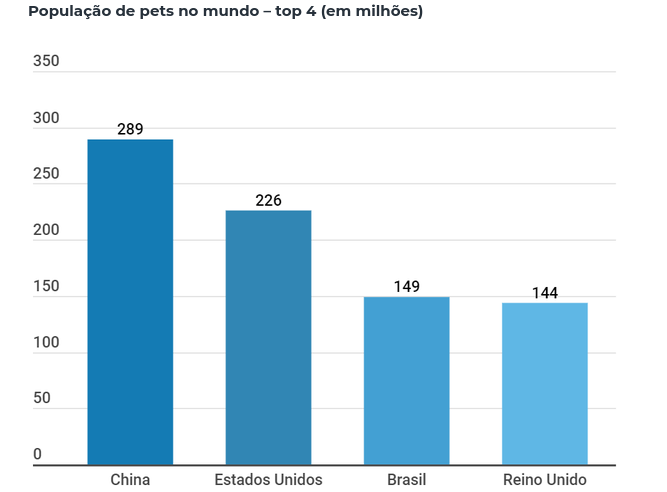
\includegraphics[
        width=0.5\linewidth,
        height=0.65\textheight,
        keepaspectratio
    ]{brasil_pets_mundo.png}
    %CORRIGIDO
    \fonte{\citeonline{panoramapetvet2023}.}
\end{figure}


%CORRIGIDO
Essa mudança de perfil social das famílias, em que o \textit{pet} passou a ser um membro de vital importância, tornou os tutores muito mais vigilantes e engajados com a transparência do cuidado do seu animal de estimação. Como consequência, todos os meios que se dedicam ao tratamento animal passaram a ser mais cautelosos com o bem-estar dos animais de estimação. A expansão da demanda por cuidados de saúde e bem-estar animal também se manifesta no ambiente de negócios. Levantamento do Sebrae, elaborado a partir de dados da Receita Federal, aponta que a abertura anual de pequenos negócios voltados ao mercado \textit{pet} passou de 12,7 mil, em 2023, para 15,5 mil, em 2025, o que corresponde a uma alta de 22\% no período \cite{sebrae2026}. No mesmo sentido, dados da Abinpet e do Instituto \textit{Pet} Brasil, divulgados por \citeonline{arbex2025}, indicam que o país ultrapassou a marca de 320 mil estabelecimentos do setor em 2024.

%CORRIGIDO
Ademais, notou-se uma mudança social expressiva no que tange à preocupação com a fauna urbana e doméstica. Essa maior consciência quanto à senciência e à valorização da vida animal reflete-se na criação e no endurecimento de arcabouços jurídicos, como a Lei Estadual nº 17.972/2024, de São Paulo, que reconhece cães e gatos como ``seres sencientes dotados de natureza biológica e emocional, passíveis de sofrimento'' \cite[art.~3º, IV]{saopaulo2024}, e a Lei Sansão (Lei nº 14.064/2020), que elevou as penas para crimes contra cães e gatos \cite{leisansao2020}, além do fortalecimento do terceiro setor (ONGs) para o acolhimento de animais vulneráveis. Esse movimento é reforçado pela atuação de organizações de proteção animal: segundo dados do Instituto \textit{Pet} Brasil, cerca de 4,8 milhões de cães e gatos vivem em situação de vulnerabilidade no país, dos quais mais de 201 mil estão sob a responsabilidade de ONGs \cite{oliveira2026}.

%CORRIGIDO
Paralelamente a essa expansão do mercado \textit{pet}, a transformação digital na saúde tem impulsionado a transição de registros físicos para sistemas de informação complexos \cite{pimazzoni2023}. No contexto da medicina veterinária, essa evolução não se limita apenas à substituição do papel, mas abrange a otimização de processos clínicos e a exigência de alta mobilidade profissional. A eficiência no diagnóstico e na conduta terapêutica está diretamente ligada à disponibilidade imediata do histórico do paciente. Contudo, essa premissa esbarra em um obstáculo técnico crítico em cenários de atendimento externo, visto que os profissionais dependem de dispositivos móveis e as aplicações atuais muitas vezes falham em suprir essa demanda operacional em locais com conexão instável ou ausente. A Figura~\ref{fig:cuidadoanimal} ilustra o cuidado clínico dispensado ao animal de estimação.

\begin{figure}[H] 
    \centering 
    %CORRIGIDO
    \caption{Ilustração do Cuidado Animal} 
    \label{fig:cuidadoanimal} 
    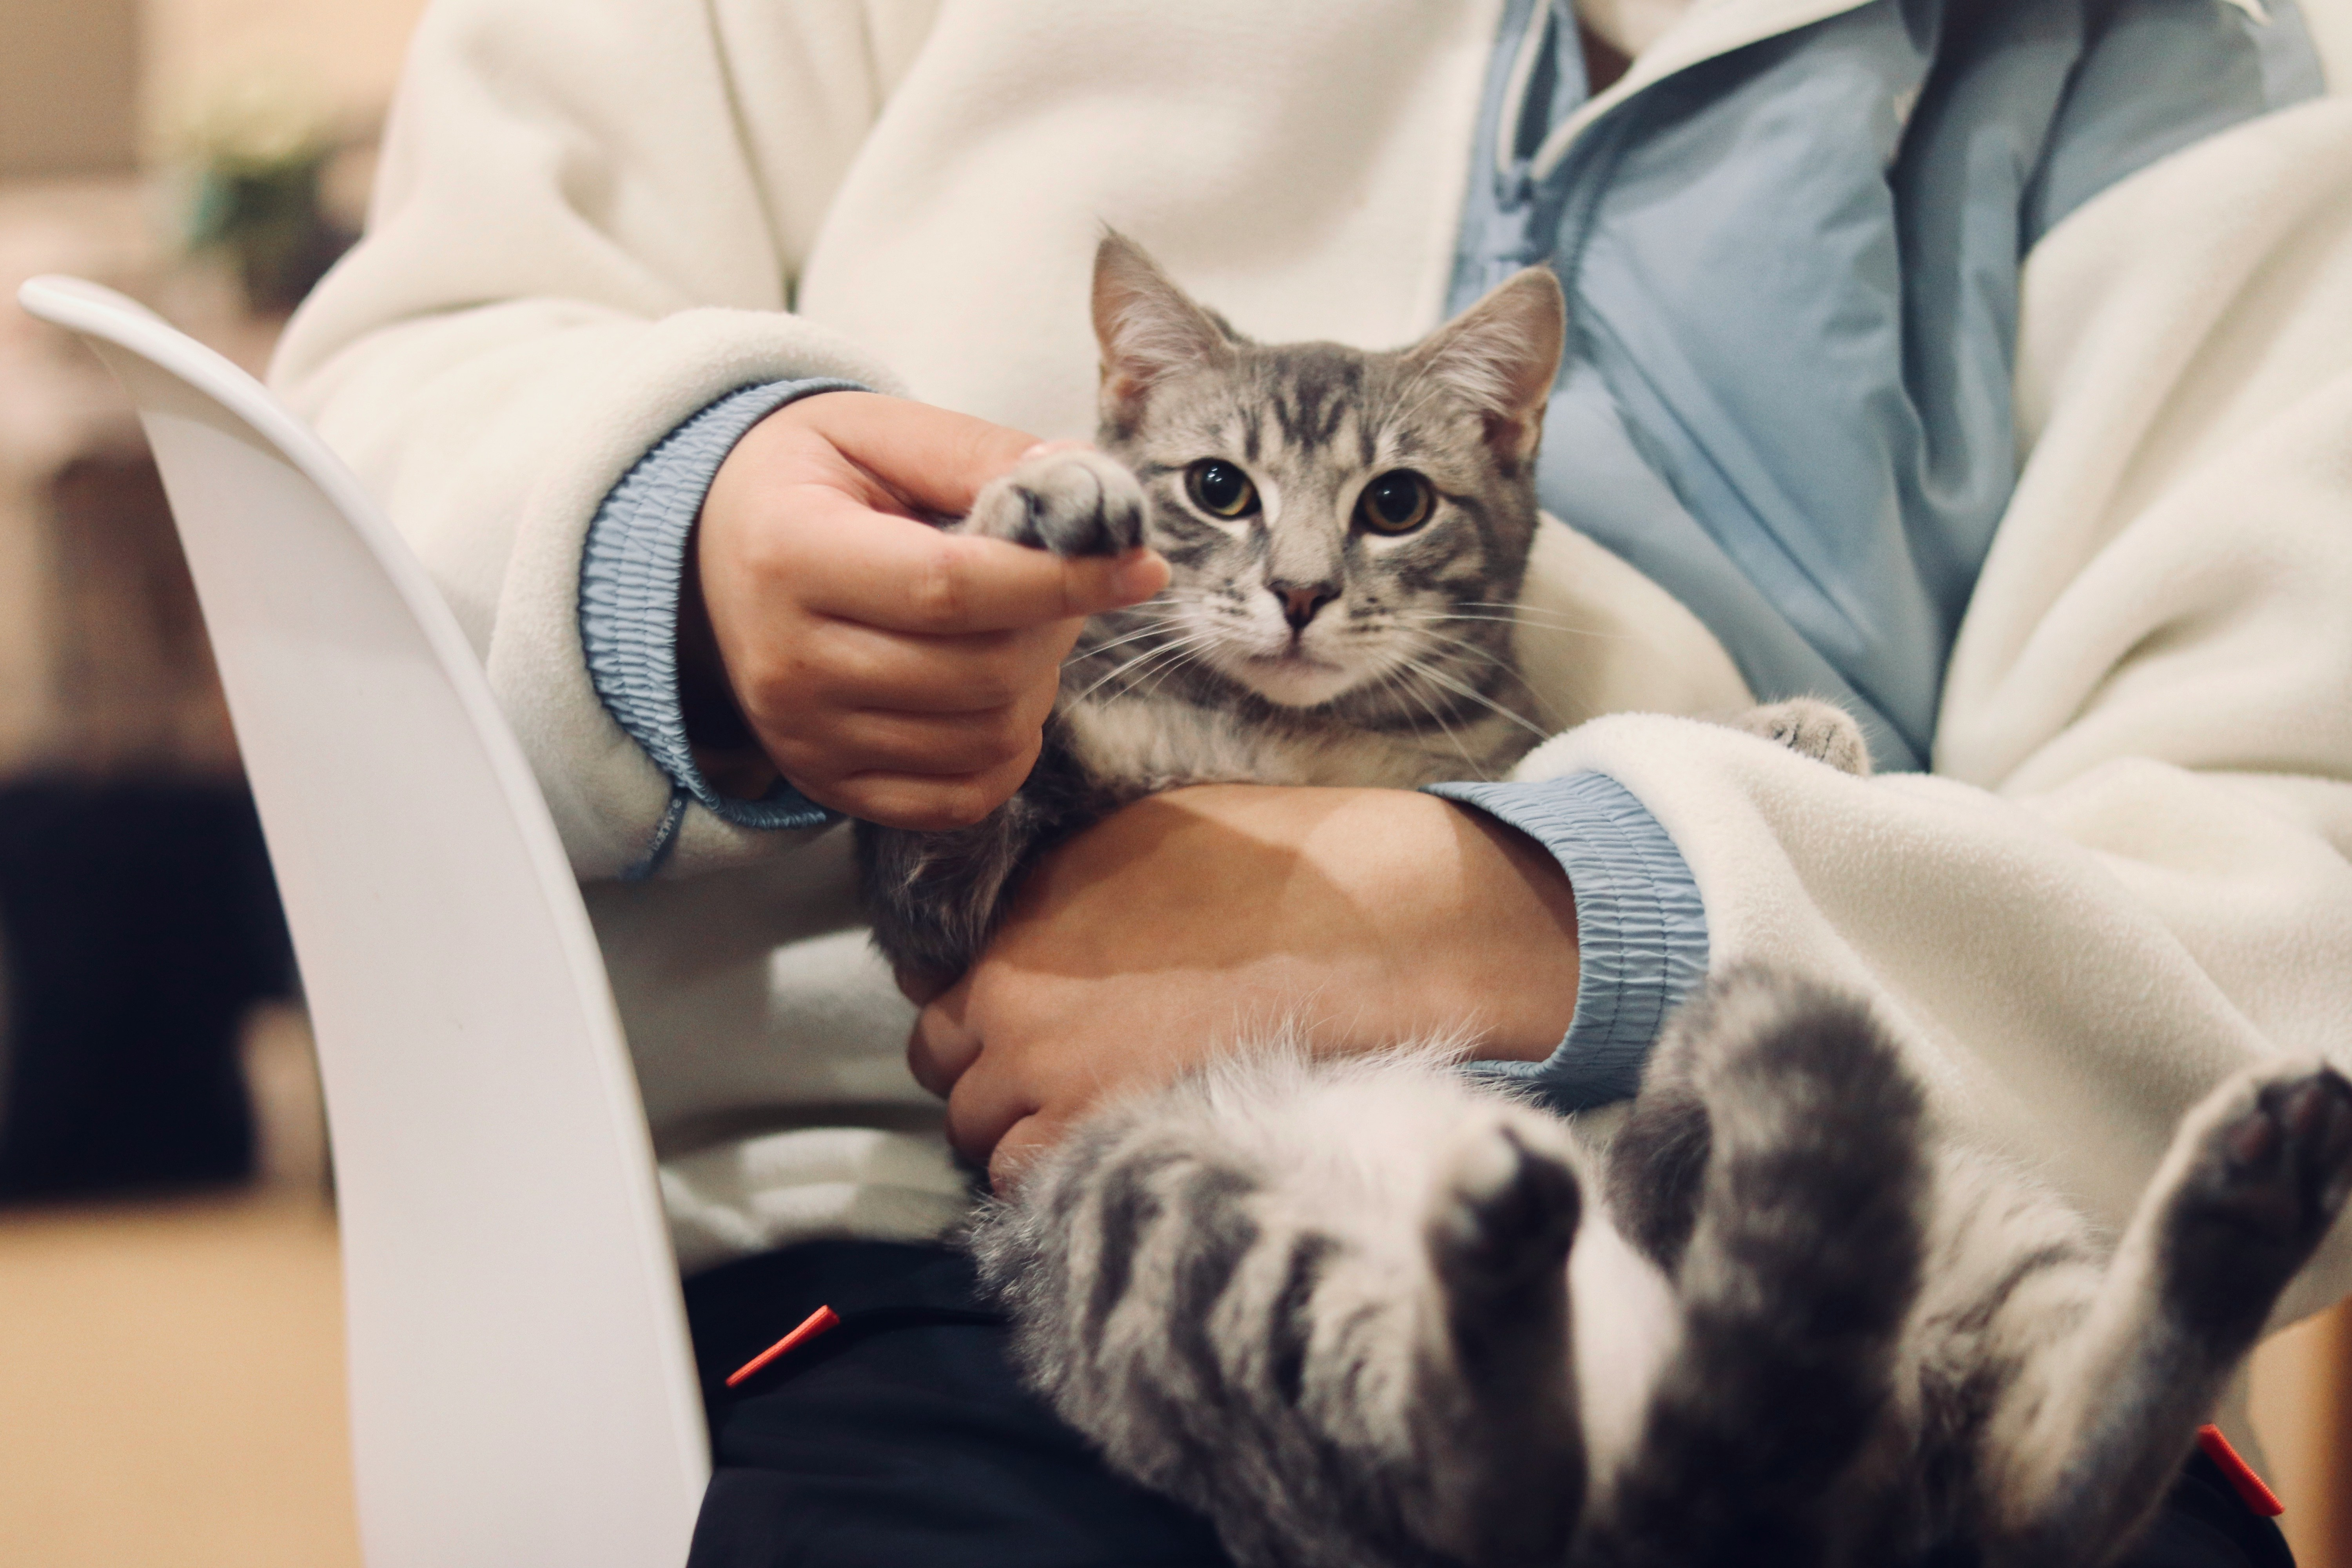
\includegraphics[
        width=0.5\linewidth,
        height=0.45\textheight,
        keepaspectratio
    ]{gato_vet.jpg}
    %CORRIGIDO
    \fonte{Werzk Luuuuuuu (\citeyear{werzk2020}).}
\end{figure}




\section{Estratégias de Persistência e o Paradigma Offline-First}
\label{sec:fundamentacao-teorica-a}
%CORRIGIDO
O conceito de \textit{offline-first} baseia-se na ideia de manipular dados quando não há conexão com a internet. Embora a maioria dos dados produzidos e compartilhados globalmente ocorra por meio da rede mundial de computadores, os sistemas \textit{offline-first} tratam a falta de conectividade não como um erro, mas como um estado previsível do sistema \cite{kleppmann2019}. Esse paradigma assume grande relevância na área de tecnologia da informação e no desenvolvimento de aplicações. Quando o foco principal de uma aplicação deixa de depender da presença de conexão com a internet, o paradigma atua como agente de persistência em sistemas desenvolvidos para operar de forma desconectada.

%CORRIGIDO
Diferentemente de sistemas que operam exclusivamente conectados e armazenam seus dados em servidores remotos, as aplicações que seguem esse paradigma utilizam o armazenamento local do dispositivo no qual são instaladas, seja um \textit{smartphone} ou um computador. Por meio da camada de cliente, com a qual o usuário interage, os dados são persistidos localmente, dessa forma, sempre que requisitados, são carregados dessa base local e exibidos ao usuário por meio de tecnologias como o \textit{WatermelonDB}, ferramenta integrada ao \textit{React Native} para a preservação de dados.

%CORRIGIDO
Embora esse modelo priorize os dados salvos localmente, a arquitetura ainda pode contar com um servidor remoto para possibilitar o funcionamento conectado. Portanto, na ausência de rede, os dados são manipulados de forma \textit{offline}, mas, quando o sinal retorna, a aplicação cliente sincroniza essas informações com o banco de dados principal, no servidor. Essa sincronização ocorre de forma assíncrona: quando a conexão é restabelecida, o sistema executa um protocolo de reconciliação para garantir que os dados inseridos localmente sejam integrados ao banco de dados principal no servidor de forma íntegra.

\section{Aspectos de Segurança e Proteção de Dados (LGPD)}
%CORRIGIDO
O crescimento constante das aplicações da área veterinária exige cuidado com a segurança do grande volume de dados gerados por seus usuários. Conforme estabelece a LGPD, Lei nº 13.709/2018 \cite{lgpd2018}, o tratamento de dados pessoais, inclusive nos meios digitais, realizado por pessoa natural ou por pessoa jurídica de direito público ou privado, deve proteger os direitos fundamentais de liberdade e de privacidade da pessoa natural. As decisões de segurança são pautadas na tríade CID (Confidencialidade, Integridade e Disponibilidade): a confidencialidade assegura que o acesso aos dados e sua divulgação ocorram somente de forma autorizada, protegendo-os, por exemplo, contra interceptações de terceiros a integridade protege os dados contra modificação ou destruição indevida e a disponibilidade garante o acesso oportuno e confiável aos dados e ao seu uso \cite[p.~2--3]{nist2017}.

%CORRIGIDO
Conforme é orientado, o tratamento dos dados coletados dos usuários será realizado somente nas hipóteses previstas no Artigo 7º da referida lei. Para a presente aplicação, consideram-se as seguintes hipóteses:

\begin{itemize}
     \renewcommand\labelitemi{-}
		%CORRIGIDO
		\item \textbf{Consentimento (Art. 7º, I):} trata da livre manifestação do usuário pela escolha do tratamento ou não tratamento dos seus dados pessoais.
		%CORRIGIDO
		\item \textbf{Cumprimento de Obrigação Legal ou Regulatória (Art. 7º, II):} justifica a coleta dos dados, quando requeridos por outras regulações, como resoluções do Conselho Federal de Medicina Veterinária (CFMV) ligadas à guarda e emissão de prontuários.
        %CORRIGIDO
        \item \textbf{Legítimo Interesse (Art. 7º, IX):} permite o tratamento dos dados quando necessário para atender aos interesses legítimos do controlador, exceto quando prevalecerem os direitos e liberdades fundamentais do titular.
	\end{itemize}

%CORRIGIDO
Além disso, vale destacar que o manuseio de dados pessoais relacionados a informações clínicas é integralmente regido pela LGPD. Em contrapartida, os dados referentes aos animais não se enquadram no escopo da Lei Geral de Proteção de Dados, portanto, qualquer informação inserida no sistema associada a um animal, como nome do \textit{pet}, espécie, raça, peso, temperatura, entre outros, é vinculada à pessoa natural que se caracteriza como seu tutor.